% !TEX encoding = UTF-8
% !TEX program = xelatex

\PassOptionsToPackage{fontset=fandol}{ctex}
\documentclass[aspectratio=169,10pt]{beamer}

\usetheme[thupurple]{thubeamer}

\graphicspath{{figures/}{../docs/thesis/figures/}}
\input{macros}

\title[AUV 海缆安全自主巡检]{%
  面向海上风电电缆运维的 AUV\\
  多源异构感知与安全自主巡检研究%
}
\author[谢冠文]{%
  \texorpdfstring{学生：谢冠文\\[2mm]导师：陈道毅\ 教授}{谢冠文，导师：陈道毅教授}%
}
\institute[清华大学]{清华大学深圳国际研究生院}
\date{硕士学位论文答辩}

\definecolor{DefenseBlue}{HTML}{276FBF}
\definecolor{DefenseGreen}{HTML}{2E8B57}
\definecolor{DefenseOrange}{HTML}{C65D12}
\definecolor{DefenseRed}{HTML}{B23A48}
\definecolor{DefenseGray}{HTML}{52606D}

\newcommand{\EvidenceTag}[1]{%
  \colorbox{DefenseBlue!12}{\strut\textcolor{DefenseBlue}{\bfseries #1}}%
}
\newcommand{\BoundaryTag}[1]{%
  \colorbox{DefenseRed!10}{\strut\textcolor{DefenseRed}{\bfseries #1}}%
}
\newcommand{\KeyNumber}[2]{%
  {\usebeamercolor[fg]{structure}\Large\bfseries #1}\\[-1mm]
  {\scriptsize #2}%
}
\newcommand{\FrameConclusion}[1]{%
  \begin{beamercolorbox}[rounded=true,sep=1mm]{block body}
    \centering\bfseries #1
  \end{beamercolorbox}%
}

\begin{document}

\begin{frame}
  \maketitle
\end{frame}

\begin{frame}{答辩主线}
  \begin{columns}[T,onlytextwidth]
    \begin{column}{0.31\textwidth}
      \begin{block}{1\quad 工程问题}
        感知质量持续变化，传统控制链却只传递状态值。
      \end{block}
    \end{column}
    \begin{column}{0.31\textwidth}
      \begin{block}{2\quad 技术路线}
        让协方差与置信度贯穿估计、决策、控制和安全执行。
      \end{block}
    \end{column}
    \begin{column}{0.31\textwidth}
      \begin{block}{3\quad 证据边界}
        用分层验证回答“何时有效、何时失效、离实物还差什么”。
      \end{block}
    \end{column}
  \end{columns}

  \vfill
  \centering
  {\Large\bfseries 核心判断：可靠自主不仅要估计状态，还要估计“状态有多可信”。}
\end{frame}

\section{问题与命题}

\begin{frame}{海缆自主巡检的核心矛盾}
  \begin{columns}[T,onlytextwidth]
    \begin{column}{0.48\textwidth}
      \begin{block}{环境与观测}
        \begin{itemize}
          \item DVL 丢包、声呐杂波、磁畸变随工况变化
          \item 多源传感器异步、频率相差一个数量级
          \item 掩埋电缆不可见，单一模态存在失效区
        \end{itemize}
      \end{block}
    \end{column}
    \begin{column}{0.48\textwidth}
      \begin{alertblock}{传统链路缺口}
        \begin{itemize}
          \item 状态估计只输出“在哪里”
          \item 决策与控制不知道“有多可信”
          \item 观测退化时仍可能维持原有控制强度
        \end{itemize}
      \end{alertblock}
    \end{column}
  \end{columns}

  \FrameConclusion{矛盾不只是“估得准不准”，而是系统能否在估计变差时主动收敛行为。}
\end{frame}

\begin{frame}{本文的可检验命题}
  \centering
  \vspace{3mm}
  {\Large
    观测质量
    \(\longrightarrow\)
    协方差
    \(\longrightarrow\)
    置信度
    \(\longrightarrow\)
    决策阈值与控制权重
  }

  \vspace{8mm}
  \begin{columns}[T,onlytextwidth]
    \begin{column}{0.31\textwidth}
      \begin{block}{H1\quad 可观测}
        扰动增强时，自适应协方差应被触发且可核查。
      \end{block}
    \end{column}
    \begin{column}{0.31\textwidth}
      \begin{block}{H2\quad 可调度}
        低置信度应改变行为优先级和控制代价。
      \end{block}
    \end{column}
    \begin{column}{0.31\textwidth}
      \begin{block}{H3\quad 有边界}
        感知完全退化时，权重调整不应被宣称仍有优势。
      \end{block}
    \end{column}
  \end{columns}

  \FrameConclusion{验证目标是“机制、收益与失效边界”同时成立，而非追求单一最优数字。}
\end{frame}

\section{系统架构}

\begin{frame}{从工程需求到可迁移方法体系}
  \centering
  \includegraphics[width=0.98\linewidth,height=0.86\textheight,keepaspectratio]
    {architecture/auv_thesis_technical_route.pdf}
\end{frame}

\begin{frame}{异步双脑：把智能与硬实时安全解耦}
  \begin{columns}[c,onlytextwidth]
    \begin{column}{0.72\textwidth}
      \centering
      \includegraphics[width=\linewidth,height=0.72\textheight,keepaspectratio]
        {architecture/auv_v2_dual_brain_async_hardware.pdf}
    \end{column}
    \begin{column}{0.25\textwidth}
      \begin{block}{Jetson / ROS2}
        估计、决策、规划与 UA-MPC
      \end{block}
      \begin{block}{PC104 / VxWorks}
        内环、驱动、看门狗与本地保护
      \end{block}
      \begin{alertblock}{分层超时}
        ROS2 管指令回退；PC104 管硬件级失联与防触底。
      \end{alertblock}
    \end{column}
  \end{columns}
\end{frame}

\section{不确定性感知}

\begin{frame}{声磁协同：连续递推与绝对约束互补}
  \begin{columns}[T,onlytextwidth]
    \begin{column}{0.30\textwidth}
      \begin{block}{高频骨架}
        IMU 约 100 Hz\\
        DVL 约 2 Hz\\[1mm]
        ES-EKF 保持连续状态
      \end{block}
    \end{column}
    \begin{column}{0.32\textwidth}
      \begin{block}{声学辅助}
        裸露、水质好：声呐主导\\
        掩埋、浑浊：质量分数下降
      \end{block}
    \end{column}
    \begin{column}{0.32\textwidth}
      \begin{block}{磁学拉回}
        DLIA 输出幅值、相位、SNR\\
        FWHM 提供垂直距离约束
      \end{block}
    \end{column}
  \end{columns}

  \vspace{4mm}
  \begin{beamercolorbox}[rounded=true,sep=2mm]{block body}
    \centering
    \[
      z_{\mathrm{mag}}
      = \frac{1}{2}v\sin\alpha\,\Delta t_{\mathrm{FWHM}},
      \qquad
      d_{\mathrm{depth}} = z_{\mathrm{mag}}-h_{\mathrm{alt}}
    \]
  \end{beamercolorbox}

  \begin{itemize}
    \item 几何时间跨度替代未知电流幅值，降低铠装衰减和姿态变化影响。
    \item SNR 与拟合残差进入 \(\boldsymbol{R}_k\)，决定磁观测应被信任到什么程度。
  \end{itemize}
\end{frame}

\begin{frame}{不确定性成为跨层调度信号}
  \centering
  \includegraphics[width=0.98\linewidth,height=0.86\textheight,keepaspectratio]
    {architecture/auv_v2_uncertainty_highway.pdf}
\end{frame}

\begin{frame}{状态估计证据：稳定输出且协方差机制被真实触发}
  \begin{columns}[c,onlytextwidth]
    \begin{column}{0.58\textwidth}
      \centering
      \includegraphics[width=\linewidth,height=0.61\textheight,keepaspectratio]
        {experiments/mag_lever_arm_fullflow_20260705_2145/02_mag_extrinsics_error_reduction.png}
      \scriptsize 仿真外参标定框架，不等同于真机转台标定。
    \end{column}
    \begin{column}{0.38\textwidth}
      \begin{block}{扰动回归}
        \centering
        \KeyNumber{24/24}{8 场景 \(\times\) 3 随机种子全部完成}
      \end{block}
      \begin{block}{自适应协方差}
        \centering
        \KeyNumber{0.24--0.36}{八类场景中的触发率范围}
      \end{block}
      \begin{block}{磁外参仿真标定}
        \centering
        \KeyNumber{96.27\% / 95.31\%}{平移误差 / 安装角误差下降}
      \end{block}
    \end{column}
  \end{columns}

  \FrameConclusion{“输出没有崩溃”与“协方差知道自己在变差”是两条独立证据。}
\end{frame}

\section{决策与控制}

\begin{frame}{行为树负责抢占，状态机负责生命周期}
  \begin{columns}[c,onlytextwidth]
    \begin{column}{0.74\textwidth}
      \centering
      \includegraphics[width=\linewidth,height=0.72\textheight,keepaspectratio]
        {architecture/auv_v2_behavior_tree_illustration.png}
    \end{column}
    \begin{column}{0.23\textwidth}
      \small
      \begin{block}{行为树}
        安全分支高优先级，每个 tick 均可抢占任务。
      \end{block}
      \begin{block}{任务状态机}
        管理搜索、确认、跟踪与返航阶段。
      \end{block}
      \begin{alertblock}{安全落点}
        回零、上浮、防触底和人工急停保持分层。
      \end{alertblock}
    \end{column}
  \end{columns}
\end{frame}

\begin{frame}{UA-MPC：置信度连续调节控制风格}
  \small
  \begin{columns}[T,onlytextwidth]
    \begin{column}{0.52\textwidth}
      \begin{beamercolorbox}[rounded=true,sep=2mm]{block body}
        \[
          J =
          \sum_{k=0}^{N-1}
          \left(
            w_{\mathrm{track}}(c)\,\lVert e_k\rVert^2
            + w_{\mathrm{u}}(c)\,\lVert \Delta u_k\rVert^2
          \right)
        \]
      \end{beamercolorbox}
      \begin{itemize}
        \item 高置信度：保持正常跟踪与控制代价。
        \item 低置信度：放大关键跟踪项，sigmoid 降低控制代价。
        \item 求解失败：显式回退 LOS/上一安全输出，不伪装为 MPC 成功。
      \end{itemize}
    \end{column}
    \begin{column}{0.43\textwidth}
      \begin{block}{机制归因}
        \textbf{主贡献：}低置信度下的 sigmoid 控制代价降权，同时改善可解性与 S 弯横向精度。
      \end{block}
      \begin{block}{参数边界}
        更线性的置信度映射仅有边际收益；默认指数与求解器迭代上限均不据此修改。
      \end{block}
      \begin{alertblock}{适用前提}
        权重调整不能替代已完全丢失的速度观测。
      \end{alertblock}
    \end{column}
  \end{columns}
\end{frame}

\begin{frame}{主消融：综合压力下双侧改善，重度丢包下失效}
  \small
  \begin{table}
    \centering
    \begin{tabularx}{\linewidth}{l>{\centering\arraybackslash}X>{\centering\arraybackslash}X>{\centering\arraybackslash}X}
      \toprule
      场景 & 水平 RMSE & 横向 RMSE & 结论 \\
      \midrule
      干净基线
        & 改善约 4.7\%
        & \(0.0038\rightarrow0.0034\) m
        & 小幅改善 \\
      重度 DVL 丢包
        & \textcolor{DefenseRed}{变差约 1.9\%}
        & UA 略差
        & \textcolor{DefenseRed}{不再有优势} \\
      综合压力
        & \textcolor{DefenseGreen}{改善约 10.4\%}
        & \textcolor{DefenseGreen}{\(0.0035\rightarrow0.0029\) m}
        & \textcolor{DefenseGreen}{改善约 15.8\%} \\
      \bottomrule
    \end{tabularx}
  \end{table}

  \vspace{3mm}
  \begin{columns}[T,onlytextwidth]
    \begin{column}{0.48\textwidth}
      \begin{block}{成立条件}
        多扰动叠加但状态估计尚未完全退化，置信度调度能形成“定位 + 控制”同向收益。
      \end{block}
    \end{column}
    \begin{column}{0.48\textwidth}
      \begin{alertblock}{不能外推}
        定位指标含离线滤波评估；不能据此单独声称完整控制性能显著优于基线。
      \end{alertblock}
    \end{column}
  \end{columns}
\end{frame}

\section{实验与证据}

\begin{frame}{负结果同样决定工程选型}
  \begin{columns}[c,onlytextwidth]
    \begin{column}{0.62\textwidth}
      \centering
      \includegraphics[width=\linewidth,height=0.64\textheight,keepaspectratio]
        {terrain_following/terrain_clearance_rmse_pid_mpc.png}
    \end{column}
    \begin{column}{0.34\textwidth}
      \begin{block}{近底地形跟随}
        三档地形、每档三种子均无安全违规；调优 PID 内层不弱于 MPC。
      \end{block}
      \begin{block}{路径跟踪}
        MPC 在长/短 S 弯和发卡路径优于或持平基线；直角折弯上 LOS 前瞻更优。
      \end{block}
      \begin{alertblock}{研究结论}
        不存在“一个控制器覆盖所有工况”的证据。
      \end{alertblock}
    \end{column}
  \end{columns}
\end{frame}

\begin{frame}{分层证据：结论强度不超过验证层级}
  \centering
  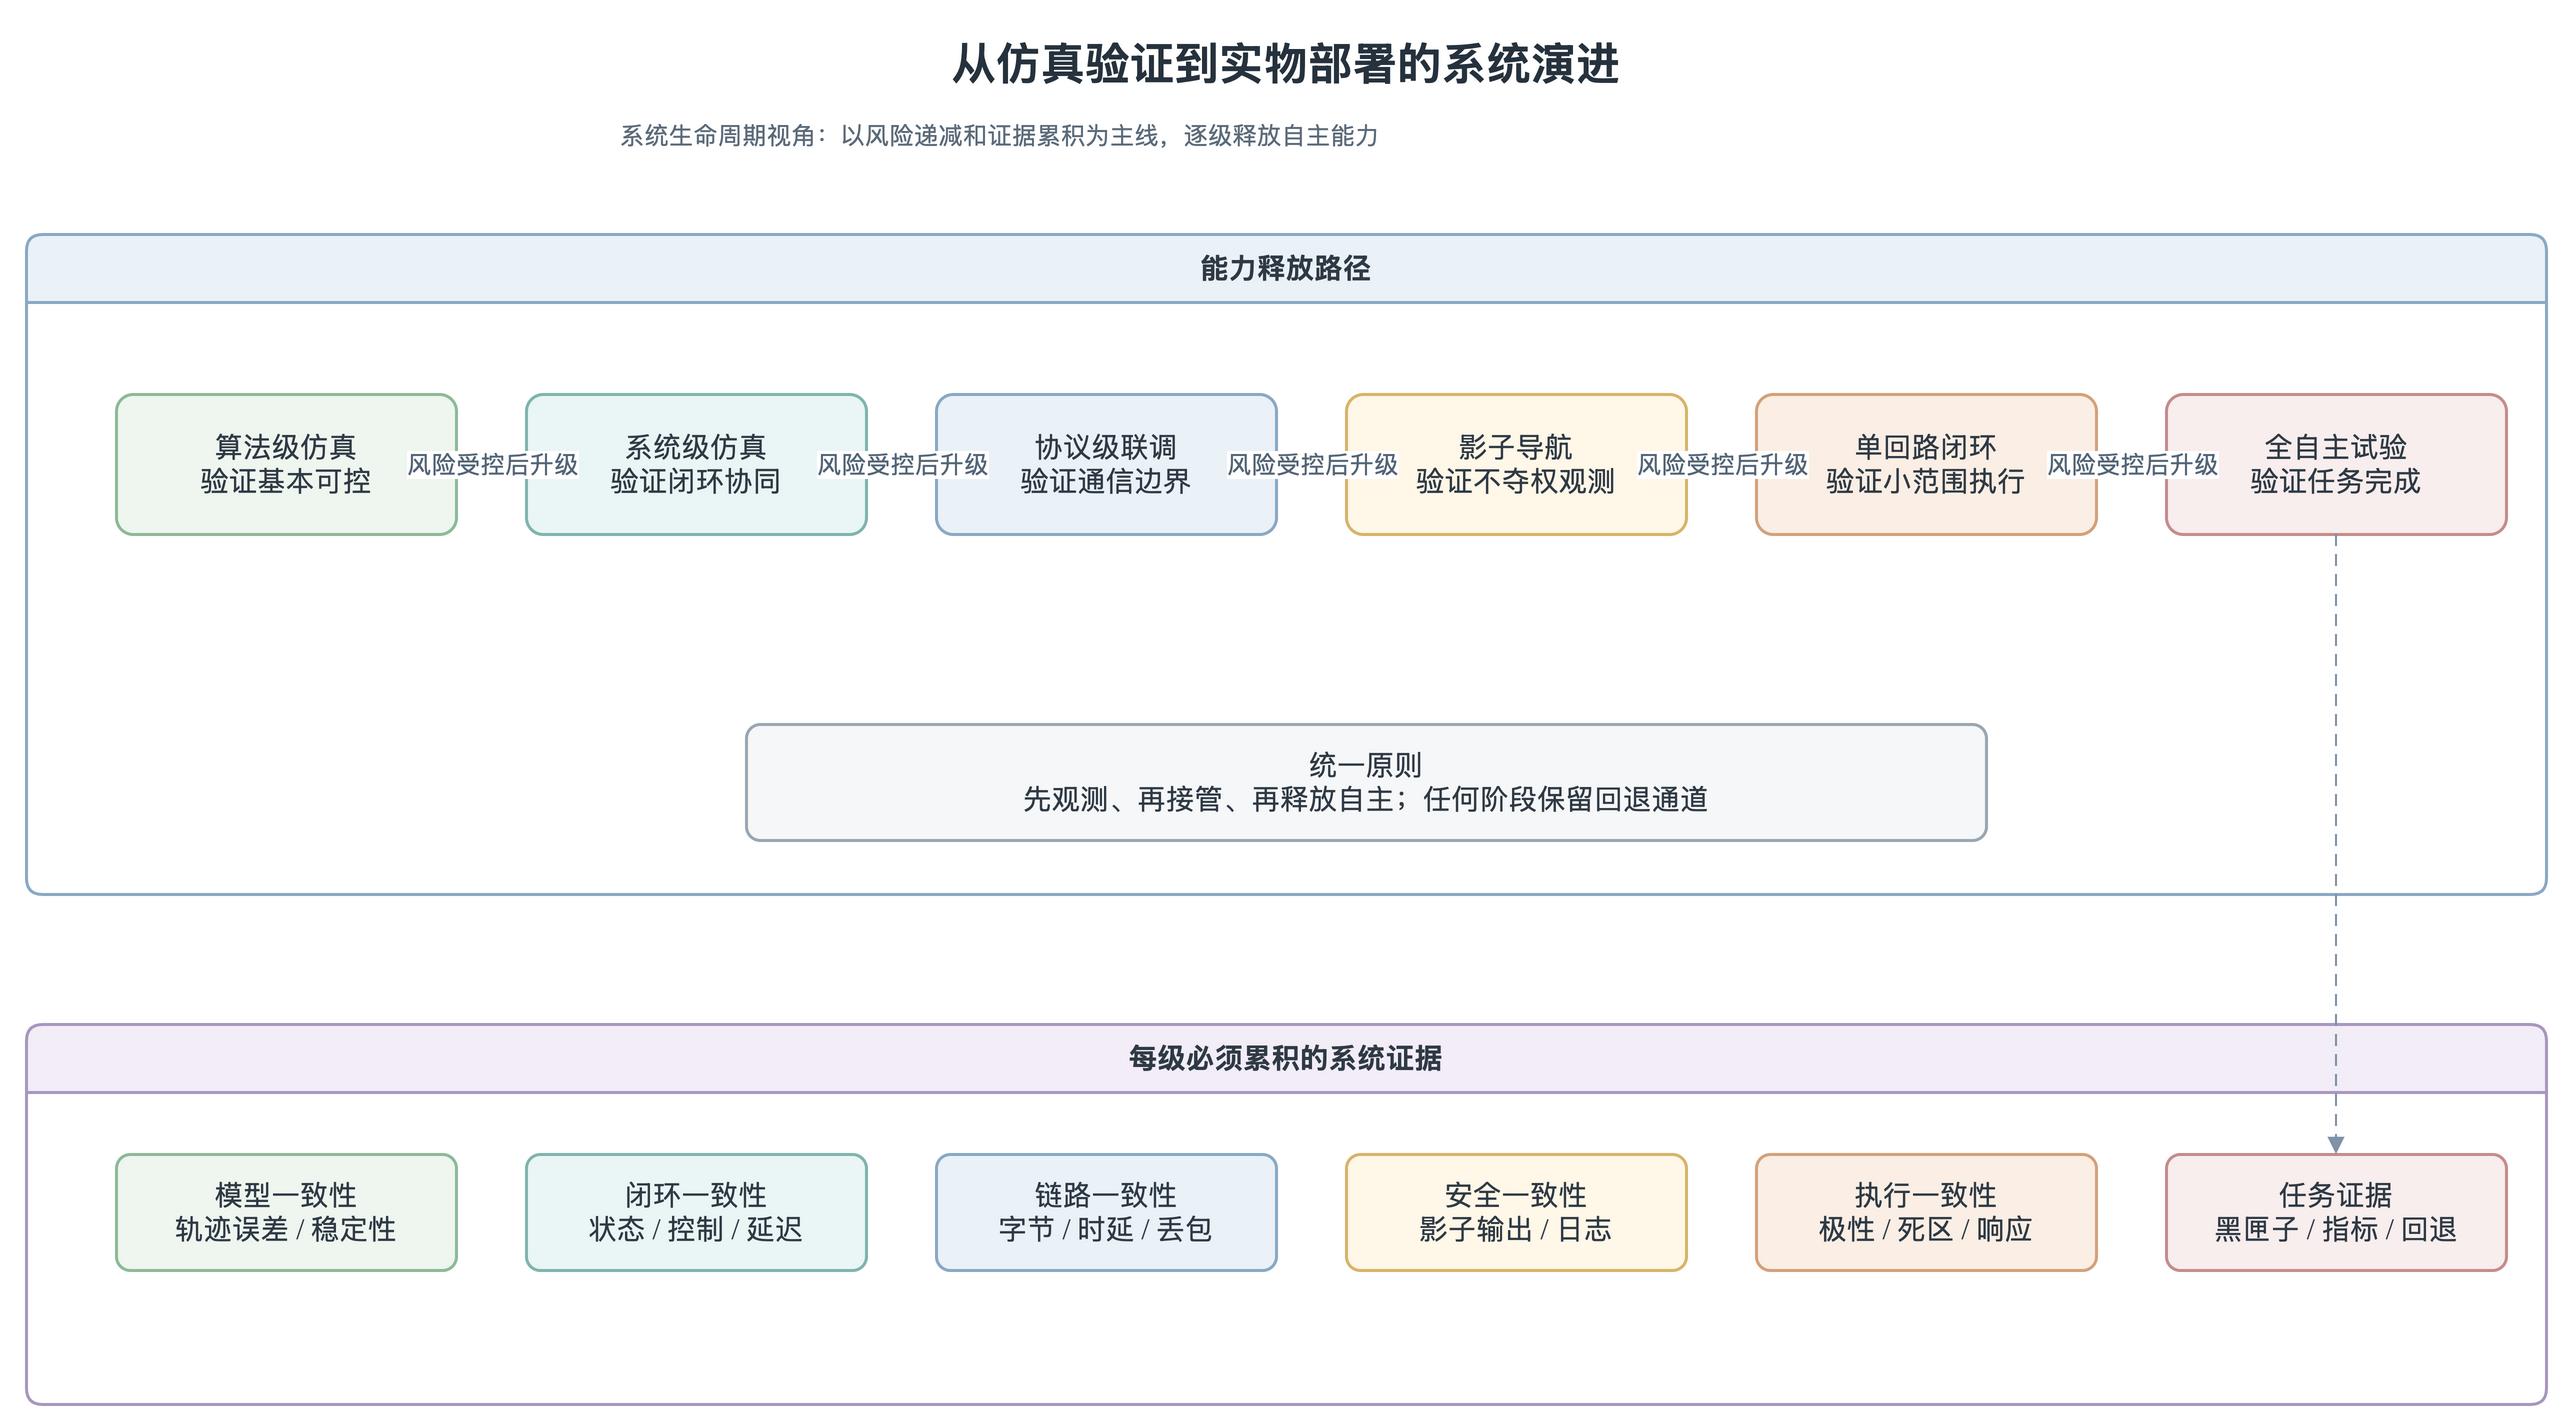
\includegraphics[width=0.88\linewidth,height=0.75\textheight,keepaspectratio]
    {architecture/auv_system_verification_deployment_ladder.png}

  \FrameConclusion{本文已闭合算法、数字孪生和部署接口证据；实物标定与海试仍是独立门槛。}
\end{frame}

\begin{frame}{从先验畸变失败到六自由度闭环恢复}
  \begin{columns}[c,onlytextwidth]
    \begin{column}{0.70\textwidth}
      \centering
      \includegraphics[width=\linewidth,height=0.62\textheight,keepaspectratio]
        {cable_acceptance/pvs_closedloop_recovery_prior_alignment.png}
    \end{column}
    \begin{column}{0.27\textwidth}
      \small
      \begin{alertblock}{先暴露失败}
        中、重档开环回放各 \(3/3\) 不通过，偏差传导至验收。
      \end{alertblock}
      \begin{block}{物理前提修复}
        磁观测被真实接受后启用在线修正；阈值不变。
      \end{block}
      \begin{block}{闭环恢复}
        中、重档各 \(3/3\) 通过；重档约 12 s 进入 \(\pm3.4\) m 廊道。
      \end{block}
      \scriptsize
      \BoundaryTag{边界}\quad 数字孪生、静态畸变、满足磁观测前提。
    \end{column}
  \end{columns}
\end{frame}

\section{结论}

\begin{frame}{贡献、结论与下一步}
  \begin{columns}[T,onlytextwidth]
    \begin{column}{0.31\textwidth}
      \begin{block}{机制贡献}
        声磁协同 ES-EKF 将观测质量映射为协方差与置信度，并跨层传递。
      \end{block}
      \centering
      \EvidenceTag{24/24 扰动运行完成}
    \end{column}
    \begin{column}{0.31\textwidth}
      \begin{block}{系统贡献}
        双脑异步、行为树抢占、任务状态机与 UA-MPC 形成分层安全闭环。
      \end{block}
      \centering
      \EvidenceTag{综合压力双侧改善}
    \end{column}
    \begin{column}{0.31\textwidth}
      \begin{block}{证据贡献}
        以失败注入、根因定位和闭环恢复定义结论成立条件，而非隐藏负结果。
      \end{block}
      \centering
      \EvidenceTag{中/重档各 3/3 恢复}
    \end{column}
  \end{columns}

  \vspace{5mm}
  \begin{alertblock}{仍需完成的实物证据}
    磁传感器九参数与工频台架标定、真实声磁噪声、真机双脑网络时延，以及湖试/海试条件下的闭环验收。
  \end{alertblock}

  \FrameConclusion{本文完成的是可解释、可验证、可迁移的自主巡检方法体系，而非提前宣称真机验收。}
\end{frame}

\begin{frame}
  \centering
  {\Huge 谢谢各位老师}\\[8mm]
  {\Large 敬请批评指正}\\[10mm]
  {\normalsize
    \textcolor{DefenseGray}{核心问题：如何让 AUV 在“不确定”时仍保持可解释的安全自主？}
  }
\end{frame}

\appendix
\section{备份}

\begin{frame}{备份：主要结果与证据边界}
  \scriptsize
  \begin{tabularx}{\linewidth}{lccX}
    \toprule
    结果 & 样本量 & 结论 & 边界 \\
    \midrule
    ES-EKF 扰动回归 & 8 场景 \(\times\) 3 种子 & 24/24 完成 & 离线仿真评估 \\
    磁外参标定 & \(n=1\) 全流程 & 96.27\% / 95.31\% & 仿真标定框架 \\
    地形跟随 & 3 档 \(\times\) 3 种子 & 零安全违规 & PVS 与真地形口径 \\
    UA-MPC 主消融 & 3 场景 \(\times\) 2 模式 \(\times\) 3 种子 & 综合压力改善 & 重度 DVL 丢包无优势 \\
    闭环先验恢复 & 中/重档各 3 次 & 各 3/3 就绪通过 & 满足磁观测物理前提 \\
    \bottomrule
  \end{tabularx}
\end{frame}

\begin{frame}{备份：分层安全时序口径}
  \small
  \begin{tabularx}{\linewidth}{lccX}
    \toprule
    层级 & 周期/阈值 & 触发对象 & 动作 \\
    \midrule
    ROS2 仲裁 & 1.0 s / 1.5 s & PC 原始指令 & 软告警 / hard ESTOP \\
    ROS2 控制 & 0.5 s & MPC 指令 & 回退安全控制输出 \\
    自治守卫 & 200 ms & 遥测新鲜度 & 拒绝过期状态与未授权任务 \\
    PC104/VxWorks & 0.1 s 周期，约 1.0 s 超时 & Jetson 有效指令 & 切回遥控、清零推进并上报告警 \\
    本地硬保护 & 实时 & 深度、近底、漏水等 & 防触底、上浮或人工干预 \\
    \bottomrule
  \end{tabularx}

  \vspace{3mm}
  \BoundaryTag{注意}\quad 不同层处理不同故障对象，不能把所有超时合并成单一数值。
\end{frame}

\begin{frame}[allowframebreaks]{参考文献}
  \nocite{dlt1278_2025}
  \bibliographystyle{thubeamer}
  \bibliography{ref/auv-references}
\end{frame}


\end{document}
